\chapter{Quark/hybrid stars}

\TODO{titles}

\TODO{units, $\hbar = c = G = k_B = 1$ or not?}

\TODO{organize project and master thesis together}

\section{Electric charge neutrality and chemical equilibrium in stars}

\TODO{generally, see Halvor's detailed discussion about this}

When we solved the Tolman-Oppenheimer-Volkoff equations for ideal neutron stars in \cref{chap:nstars}, our lives were quite simple.
The stars consisted of only one charge neutral particle, and we simply eliminated its chemical potential to find the equation of state.
Now we will consider stellar models with a greater variety of particles and non-zero electric charge.

How do we now find the equation of state, when there is one chemical potential for each kind of particle?
The answer is to impose additional physical requirements of electric charge neutrality and chemical equilibrium.
With these conditions, we will relate all but one of the chemical potentials to each other, leaving only one independent variable that we will eliminate to find the equation of state.

\subsection{Global electric charge neutrality}

We can make a very simple classical argument for why there can be no \emph{global} net electric charge in stars by comparing Newton's law of gravity and Coulomb's law.
Consider a test particle of mass $m$ and electric charge $q$ on the surface $R$ from the center of a star with total mass $M$ and electric charge $Q$.
In an idealized situation, the test particle is affected by the gravitational and electrostatic force, so that the total outwards \TODO{radial?} force on it is
\begin{equation}
	F_\text{out} = -G \frac{M m}{R^2} + k_e \frac{Q q}{R^2} .
\end{equation}
Furthermore, suppose the star consists of $N$ particles weighing \TODO{weight $\rightarrow$ mass} no more than some heavy baryon with mass $m_B$, so $M < N M_B$ and $m < m_B$.
Any electrically charged particle has about one elementary charge $q \approx \pm e$.
If the star has an opposite charge $Q = \mp Z e$, then $F_\text{out} < 0$ and the test particle stays in the star.
On the other hand, if the star has a like charge $Q = \pm Z e$, then
\begin{equation}
	F_\text{out} > -G \frac{N m_B^2}{R^2} + k_e \frac{Z e^2}{R^2} .
\end{equation}
We then surely have $F_\text{out} > 0$, provided that the number of elementary charges per particle satisfies
\begin{equation}
	\frac{Z}{N} > \frac{G m_B^2}{k_e e^2} \approx 10^{-37} ,
\end{equation}
where we have assumed a typical baryon mass $m_B = m_p = \SI{1.67e-27}{\kilogram}$.
This corresponds to practically zero electric charge per particle in the star.

This means that particle are expelled from the star while $Z > 10^{-37} N$ until $Z$ has fallen to \emph{at least} $Z < 10^{-37} N$.
We conclude that for all practical purposes, stars are \emph{globally} electrically charge neutral.

\TODO{what about radius $r < R$ instead of $r=R$?}

\TODO{what about general relativity instead of Newtonian gravity?}

\TODO{what about contribution from pressure and other things to $F_\text{out}$?}

\TODO{can I recast inequality in charge per solar mass? see discussion at beginning of \url{www.if.ufrgs.br/hadrons/MMalheiro.pdf}}

\subsection{Local electric charge neutrality}

\TODO{non-understandable comment from Møte 4, Gibbs/Maxwell contstruction etc?}

\TODO{Glendenning has papers regarding local charge neutrality (?)}

The argument in the previous section shows that a star can have no \emph{total} electric charge, but it places absolutely no limitations on its \emph{distribution}.
Moreover, our approach to calculating equations of state is inherently \emph{local} -- we obtain the equation of state $\epsilon(P)$ by eliminating the density $n$ at any \emph{single point} from the energy density $\epsilon(n)$ and pressure $P(n)$.
To make use of electric charge neutrality in our approach, we will promote it from a \emph{global} constraint to a \emph{local} one.

\TODO{now explain...}

\TODO{TOV equation is derived by assuming ideal fluid in equilibrium -- would local charge destroy that?}

\TODO{draw inspiration from standard argument that $\vec{E} = 0$ everywhere inside a conductor?}

Satisfied by
\begin{equation}
	\sum_p q_p \, n(\mu_p) = 0 ,
\end{equation}
where the sum is over all particles present, each with electric charge $q_p$.
In the zero-temperature approximation with the density \eqref{eq:nstars:density_zeroT}, this is satisfied if
\begin{equation}
	\sum_p q_p \left( \mu_p^2 - m_p^2 \right)^{3/2} = 0 .
\end{equation}

\subsection{Chemical equilibrium}

\TODO{introduce}

Important reactions
\begin{subequations}
\begin{align}
	d     &\leftrightarrow u + e + \bar{\nu}_e, \\
	s     &\leftrightarrow u + e + \bar{\nu}_e, \\
	s + u &\leftrightarrow u + d .
\end{align}
\end{subequations}
Assume neutrinos leave star \TODO{why?}.
Then chemical equilibrium implies
\begin{subequations}
\begin{align}
	\mu_d &= \mu_u + \mu_e, \\
	\mu_s &= \mu_u + \mu_e, \\
	\mu_s &= \mu_u .
\end{align}
\end{subequations}
(the third follows automatically from the two first)

\section{Linear sigma model}

\begin{figure}
\centering
\tikzsetnextfilename{potential}
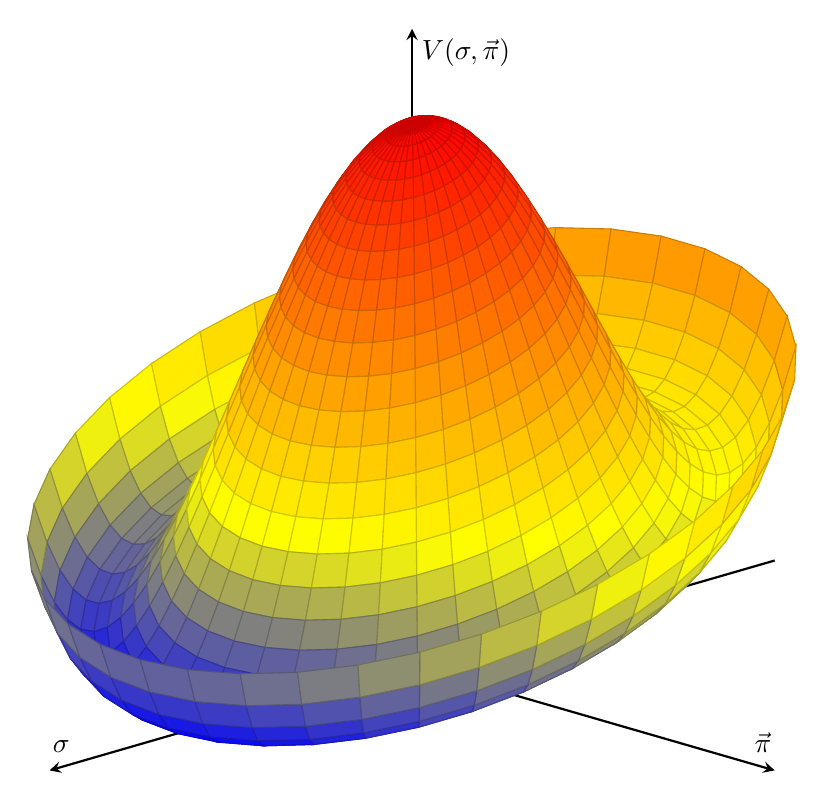
\begin{tikzpicture}
\begin{axis}[
	width = 20cm, height=15cm,
	%title = {Potential},
	xlabel = $\sigma$, ylabel = $\vec\pi$, zlabel = {$V(\sigma,\vec\pi)$},
	xmin=-4.0, xmax=+4.0, ymin=-4.0, ymax=+4.0, zmin=0, zmax=2.2,
	xtick=\empty, ytick=\empty, ztick=\empty,
	axis lines=center,
	axis line style = thick,
	view={135}{25},
	%colormap/blackwhite, mesh/interior colormap name=plasmarev,
]
	\addplot3 [surf, thin, domain=0:3.0, domain y=0:2*pi, samples=30, samples y=40, z buffer=sort] ({x*cos(deg(y))},{x*sin(deg(y))},{-1/2*((x*cos(deg(y)))^2+(x*sin(deg(y)))^2) + 1/24*((x*cos(deg(y)))^2+(x*sin(deg(y)))^2)^2 + 3/2 - 0.15*x*cos(deg(y)) + 0.15*sqrt(6)});
	%\addplot3 [domain=0:2*pi, samples=50, samples y=1] ({sqrt(6)*cos(deg(x))},{sqrt(6)*sin(deg(x))},{0});
\end{axis}
\end{tikzpicture}
\caption{\label{fig:lsm:potential}%
	A two-dimensional realization of the potential \eqref{eq:lsm:potential} looks like a Mexican hat, tilted along the $\sigma$-axis by the explicit symmetry breaking parameter $h$.
	If $h = 0$, the hat is upright with an infinite number of minima around $\sigma^2 + \vec\pi^2 = 6m^2 / \lambda$.
	If $h \neq 0$, the hat is tilted and has a global minimum at $\vec\pi = 0$ and $\sigma = \avg{\sigma}$ determined by \eqref{eq:lsm:ground_state_implicit}.
}
\end{figure}

\TODO{justify this effective MODEL from QCD. Expand QCD $\lagr$ at low energy?}

The Lagrangian density for the linear sigma model coupled to quarks is
\begin{equation}
	\lagr = \sum_{c=1}^{N_c} \bar{q}_c \Big[ i \slashed\partial + \mu \gamma^0 - g \left( \sigma + i \gamma^5 \vec\tau \cdot \vec\pi \right) \Big] q_c
	      + \frac12 \left[ \left( \partial_\mu \sigma \right)^2 + \left( \partial_\mu \vec\pi \right)^2 \right] - \pot(\sigma,\vec\pi) ,
\label{eq:lsm:lagrangian}
\end{equation}
with the potential
\begin{equation}
	\pot(\sigma,\vec\pi) = \frac12 m^2 \left( \sigma^2 + \vec\pi^2 \right) + \frac{\lambda}{4!} \left( \sigma^2 + \vec\pi^2 \right)^2 - h \sigma .
	                     % = \frac{\lambda}{4!} \left( \sigma^2 + \vec\pi^2 - \frac{6m^2}{\lambda} \right)^2 -\frac{3 m^4}{2 \lambda} .
\label{eq:lsm:potential}
\end{equation}
Here $q_c = [u_c, d_c]^T$ represents quarks of the $N_c = 3$ colors red, green and blue and the $N_f = 2$ flavors up and down, so $(q_c)_f$ make up a total of $N_c \times N_f = 6$ Dirac spinors.
In addition, $\sigma$ and $\vec\pi = [\pi^+, \pi^0, \pi^-]^T$ are four bosonic scalar fields representing sigma and pion mesons.
At this point, the quarks are massless Dirac fermions whose conserved charge densities $j^0 = \bar\psi \gamma^0 \psi$ are coupled to chemical potentials $\mu = \diag(\mu_u, \mu_d)$, interacting with a Yukawa coupling of strength $g$ that models the strong force \TODO{non-mentioned comment in Møte 4}, where $\vec\tau$ are the Pauli matrices \eqref{eq:tft:pauli_matrices}.
\TODO{write $(\sigma, \vec\pi)^T$ as 4-vector and mention $O(4)$ symmetry, explain from $SU(2)_L$, $SU(2)_R$, etc.?}

To make sense of this theory, we must investigate how it behaves around the classical ground state of the potential \eqref{eq:lsm:potential}.
As shown in \cref{fig:lsm:potential}, the potential is shaped like a tilted Mexican hat with a classical ground state at $\sigma = \avg{\sigma} \neq 0$ and $\pi = \vec\pi = 0$.
Hence, the value of $\avg{\sigma}$ is determined implicitly by
\begin{equation}
	\pdv{\pot}{\sigma}_{(\sigma,\vec\pi)=(\avg{\sigma},\vec{0})} = m^2 \avg{\sigma} + \frac{\lambda}{6} \avg{\sigma}^3 - h = 0 .
\label{eq:lsm:ground_state_implicit}
\end{equation}
We account for quantum fluctuations around the classical ground state by shifting
\begin{equation}
	\sigma \rightarrow \Avg{\sigma} + \tilde{\sigma}
	\qquad \text{and} \qquad
	\vec\pi \rightarrow \Avg{\vec\pi} + \tilde{\vec\pi}.
\end{equation}
In terms of the new fields $\tilde\sigma$ and $\tilde{\vec\pi}$, the Lagrangian \eqref{eq:lsm:lagrangian} is now
\begin{equation}
	\lagr = \sum_{c=1}^{N_c} \bar{q}_c \Big[ i \slashed\partial - m_q + \mu \gamma^0 - g \left( \tilde{\sigma} + i \gamma^5 \vec\tau \cdot \vec\pi \right) \Big] q_c
	      + \frac12 \left[ \left( \partial_\mu \tilde{\sigma} \right)^2 + \left( \partial_\mu \tilde{\vec\pi} \right)^2 \right] - \tilde{\pot}(\tilde{\sigma},\tilde{\vec\pi}) , %\pot(\avg{\sigma}+\tilde{\sigma},\avg{\vec\pi}+\tilde{\vec\pi}) ,
\end{equation}
where the quark fields $q$ have acquired effective masses
\begin{equation}
	m_q = g \avg{\sigma} .
\label{eq:lsm:mass_quark}
\end{equation}
The potential up to second order in the shifted fields is
\begin{equation}
\begin{split}
	\tilde{\pot}(\tilde{\sigma},\tilde{\vec\pi}) &= \pot(\avg{\sigma}+\tilde{\sigma},\avg{\vec\pi}+\tilde{\vec\pi}) \\
	                                             &\taylor \frac12 m^2 \avg{\sigma}^2 + \frac{\lambda}{4!} \avg{\sigma}^4 - h \avg{\sigma} + \frac12 m_\sigma^2 \sigma^2  + \frac12 m_\pi^2 \vec\pi^2 ,
	%V(\sigma, \vec\pi) \taylor -\frac12 m^2 \avg{\sigma}^2 + \frac{\lambda}{4!} \avg{\sigma}^4 + \frac12 (\sqrt{2} m)^2 \sigma^2 .
	%V(\sigma, \vec\pi) \taylor -\frac{3 m^4}{2 \lambda} + \frac12 (\sqrt{2} m)^2 \sigma^2 .
\label{eq:lsm:potential_shifted}
\end{split}
\end{equation}
where the $\sigma$ and $\vec\pi$ fields have acquired the effective masses
\begin{subequations}
\begin{align}
	m_\sigma^2 &= \pdv[2]{\pot}{\sigma}_{(\sigma,\vec\pi)=(\avg{\sigma},\vec{0})} = m^2 + \frac{\lambda}{2} \avg{\sigma}^2 \equalexplabove{\text{by \eqref{eq:lsm:ground_state_implicit}}} \frac{3h}{\avg{\sigma}} - 2 m^2 , \label{eq:lsm:mass_sigma} \\
	m_\pi^2    &= \pdv[2]{\pot}{\pi   }_{(\sigma,\vec\pi)=(\avg{\sigma},\vec{0})} = m^2 + \frac{\lambda}{6} \avg{\sigma}^2 \equalexplbelow{\text{by \eqref{eq:lsm:ground_state_implicit}}} \frac{h}{\avg{\sigma}} , \label{eq:lsm:mass_pi}
\end{align}%
\label{eq:lsm:mass_sigmapi}%
\end{subequations}%
The linear sigma model is an effective low-energy model of quantum chromodynamics, so accordingly we should take it seriously only in terms of the shifted fields around the stable ground states, and not in terms of the unshifted fields around the unstable equilibrium at the top of the Mexican hat.

Although we have and will continue to assume $h \neq 0$ in general, this is an excellent time to reflect upon the special case $h = 0$.
In this case, the potential \eqref{eq:lsm:potential} is symmetric under rotations in $O(4)$ of the field vector $(\sigma, \vec\pi)^T$.
This corresponds to movement along the ``brim'' of \emph{continuous} minima satisfying $\sigma^2 + \vec\pi^2 = -6 m^2 / \lambda$ in a flattened Mexican hat in \cref{fig:lsm:potential}.
\TODO{number of generators $=$ number of massless Goldstone bosons, $O(4)$ or $SO(4)$}
Upon choosing \emph{one} minima where $\sigma = \avg{\sigma} \neq 0$ and $\vec\pi = \avg{\vec\pi} = 0$, the symmetry would be broken to rotations of only the three $\vec\pi$ fields, and three massless Goldstone bosons would appear.
With $h \neq 0$, however, the $O(4)$ symmetry is explicitly broken, and \cref{eq:lsm:mass_pi} says $h = m_\pi^2 \avg{\sigma}$.
This is essentially Goldstone's theorem -- if $h = 0$, then $m_\pi = 0$ to ensure $\avg{\sigma} \neq 0$; but if $h \neq 0$, then $m_\pi \neq 0$.
Moreover, the smaller the value of $h$, the smaller the value of $m_\pi$, so the if $h$ is \emph{small}, the spontaneous symmetry breaking is \emph{approximate}, and the $\vec\pi$ fields are \emph{light}, but not massless.
\TODO{refine this messy paragraph}

We determine the four parameters $g$, $h$, $m$ and $\lambda$ in the original Lagrangian \eqref{eq:lsm:lagrangian} by comparing the four \emph{effective} quantities $\avg{\sigma}$, $m_\pi$, $m_\sigma$ and $m_q$ to the measurements
\begin{subequations}
\begin{alignat}{2}
	\avg{\sigma} &= \SI{93}{\mega\electronvolt}  &\qquad& \text{(\TODO{source}), \TODO{distinguish $\avg{\sigma}$ and $f_\pi$}}, \label{eq:lsm:fpi} \\
	m_\pi        &= \SI{138}{\mega\electronvolt} &\qquad& \text{(\TODO{source})}, \\
	m_\sigma     &= \SI{900}{\mega\electronvolt} &\qquad& \text{(in range $\SI{400}{\mega\electronvolt} < m_\sigma < \SI{700}{\mega\electronvolt}$, by \cite{ref:pdg_review_2021}) \TODO{rev}}, \\
	m_q          &= \SI{300}{\mega\electronvolt} &\qquad& \text{(by) \TODO{}}.
\end{alignat}
\end{subequations}
By inverting equations \eqref{eq:lsm:ground_state_implicit}, \eqref{eq:lsm:mass_sigmapi} and \eqref{eq:lsm:mass_quark}, we find the parameters
\begin{subequations}
\begin{align}
	g       &= \frac{m_q}{\avg{\sigma}}                 , \\ % &\qquad& \text{(by \eqref{eq:lsm:mass_quark})} , \\
	h       &= m_\pi^2 \avg{\sigma}                     , \\ % &\qquad& \text{(by \eqref{eq:lsm:mass_pi})} , \\
	m^2     &= \frac{3m_\pi^2 - m_\sigma^2}{2}          , \\ % &\qquad& \text{(by \eqref{eq:lsm:mass_sigma})} , \\
	\lambda &= \frac{3 m_\sigma^2 - 3 m_\pi^2}{f_\pi^2} .    % &\qquad& \text{(by \eqref{eq:lsm:ground_state_implicit})} .
\end{align}
\end{subequations}

According to what we learned in \cref{chap:tft} in \cref{eq:tft:boson_partition_function_momentum_out} and \eqref{eq:tft:dirac_partition_function_first},
the exact partition function corresponding to this theory is obtained by a path integral over periodic bosonic fields and anti-periodic fermionic fields, weighted by a Euclidean action in imaginary time:
\begin{equation}
	Z = \oint_- \pathintdif \bar{q} \oint_- \pathintdif q \oint_+ \pathintdif \sigma \oint_+ \pathintdif \vec\pi \exp \left\{ \int_0^\beta \dif \tau \int_V \dif^3 x \, \lagr_E[\bar{q}, q, \sigma, \vec\pi]  \right\} .
\end{equation}
As before, we are interested in $\log Z$ so we can calculate the thermodynamic quantities \eqref{eq:tft:average_quantities} and ultimately an equation of state $\epsilon(P)$, so we can solve the Tolman-Oppenheimer-Volkoff equation \eqref{eq:tov:tovsys}.
Here we will account for quantum effects of the quarks by treating them up to quadratic order (or one-loop),
but calculate only to zeroth order (or tree-level) in the meson fields and hence consider them only at the classical level.
\TODO{this is an \emph{exact} approximation as $N_c \rightarrow \infty$, because in the $\log Z$ we find below, the boson terms are $\propto N_c^0$, while the quark terms are $\propto N_c^1$}
The partition function then reads
\begin{equation}
\begin{split}
	Z &\taylor \oint_- \pathintdif \bar{q} \oint_- \pathintdif q \\
	  &\times  \exp \left\{ \int_0^{\beta} \dif \tau \int_V \dif^3 x \left[ \sum_{c=1}^{N_c} \bar{q}_c \left( i \slashed\partial -m_q + \mu \gamma^0 \right) q_c - \frac12 m^2 \avg{\sigma}^2 - \frac{\lambda}{4!} \avg{\sigma}^4 + h \avg{\sigma} \right] \right\} \\
	  &=       \prod_{f=1}^{\smash{N_f}} \prod_{c=1}^{\smash{N_c}} \oint_- \pathintdif \bar{q}_f^c \oint_- \pathintdif q_f^c \\
	  &\times  \exp \left\{ \int_0^{\beta} \dif \tau \int_V \dif^3 x \left[ \sum_{f=1}^{\smash{N_f}} \sum_{c=1}^{N_c} \bar{q}_f^c \left( i \slashed\partial - m_q + \mu_f \gamma^0 \right) q_f^c - \frac12 m^2 \avg{\sigma}^2 - \frac{\lambda}{4!} \avg{\sigma}^4 + h \avg{\sigma} \right] \right\}.
\end{split}
\end{equation}
The two last terms in the exponential are independent of the fields, so
\begin{equation}
\begin{split}
	\log Z &= -\frac12 \beta V m^2 \avg{\sigma}^2 - \frac{\lambda}{4!} \beta V \avg{\sigma}^4 + \beta V h \avg{\sigma} \\
	       &+ \sum_{f=1}^{N_f} \sum_{c=1}^{N_c} \log \oint_- \pathintdif \bar{q}_f^c \oint_- \pathintdif q_f^c \exp \left\{ \int_0^\beta \dif \tau \int_V \dif^3 x \, \bar{q}_f^c (i \slashed\partial + \mu_f \gamma^0 - m_q) q_f^c \right\} .
\end{split}
\end{equation}
We have already calculated the path integral in the last term from \cref{eq:tft:dirac_partition_function_first} to \cref{eq:tft:dirac_partition_function}!
Here, we get an additional factor $\sum_{c=1}^{N_c} = N_c$ from the color sum because the summand is independent of $c$,
while the flavor sum $\sum_{f=1}^{\smash{N_f}}$ yields $N_f$ terms that differ only by the unique chemical potentials $\mu_f$ associated with each quark flavor. 
Thus, we obtain
\begin{equation}
\begin{split}
	\log Z &= -\frac12 \beta V m^2 \avg{\sigma}^2 - \frac{\lambda}{4!} \beta V \avg{\sigma}^4 + \beta V h \avg{\sigma} \\
	       &+ 2 V N_c \sum_{f=1}^{N_f} \int \frac{\dif^3 p}{(2 \pi)^3} \left\{ \beta E(\vec{p}) + \log \left[ e^{-\beta (E(\vec{p}) - \mu_f)}+1 \right] + \log \left[ e^{-\beta (E(\vec{p}) + \mu_f)} + 1\right] \right\} ,
\end{split}
\label{eq:lsm:potential_divergent_logz0}
\end{equation}
where the dispersion \TODO{comment Møte 4?} relation is now
\begin{equation}
	E(\vec{p}) = \sqrt{p^2 + m_q^2} .
\end{equation}
Like in \cref{chap:nstars}, we assume that the chemical potentials are chosen so that anti-particles are more or less absent, so we drop their contribution in the last term in the second line.
From the middle term in the second line, we obtained the contribution $\log Z = \beta V P$ with the pressure \eqref{eq:nstars:pressure_zeroT} after taking the zero-temperature approximation.
\TODO{justify validity of zero-temperature approximation with the new masses? no, can really only do this in a retrospective way, since I don't know a priori what the temperature is inside an unknown quark star}
This time, however, we will renormalize the infinite vacuum contribution from the first term in the second line, instead of simply dropping it, like we did back in \cref{chap:nstars}.
Thus, we obtain
\begin{equation}
\begin{split}
	\log Z &= -\frac12 \beta V m^2 \avg{\sigma}^2 - \frac{\lambda}{4!} \beta V \avg{\sigma}^4 + \beta V h \avg{\sigma} + N_c N_f \log Z_0 \\
	       &+ N_c \frac{m_q^4 \beta V}{24 \pi^2} \sum_{f=1}^{N_f} \left[ (2 x_f^3 - 3x_f) \sqrt{x_f^2 + 1} + 3 \asinh x_f \right],
\end{split}
\end{equation}
where $x_f = p_f / m_q$ are normalized Fermi momenta, $\mu_f = \smash{\sqrt{p_f^2 + m_q^2}}$ are Fermi energies and the vacuum contribution is
\begin{equation}
	\log Z_0 = 2 \beta V \int \frac{\dif^3 p}{(2 \pi)^3} \sqrt{p^2 + m_q^2 } .
\label{eq:lsm:vacuum_contribution_3dim}
\end{equation}
To renormalize the vacuum contribution, let us use dimensional regularization in the minimal subtraction scheme \TODO{?}.
In $d = 3 - 2 \epsilon$ spatial dimensions, the vacuum contribution is
\TODO{can I do this in a more ``well-defined way'' by rescaling the momentum instead, like $p' = p / \Lambda^{(1-3/d)}$ where $\unit{p} = \unit{\Lambda}$, so $\unit{\dif^d p'} = \unit{\dif^3 p}$, so $\log Z$ remains dimensionless.?}
\begin{equation}
\begin{split}
	\log Z_0 &= 2 \beta V \Lambda^{3-d} \int \frac{\dif^d p}{(2 \pi)^d} \sqrt{p^2 + m_q^2} \\
	         &= 2 \beta V \Lambda^{3-d} \frac{2 \pi^{d/2}}{\Gamma(d/2)} \int_0^\infty \frac{\dif p \, p^{d-1}}{(2 \pi)^d} \sqrt{p^2 + m_q^2} .
\end{split}
\label{eq:lsm:vacuum_contribution_ddim}
\end{equation}
\TODO{what happens to the dimensions of the potential $V$ (as consequence of requiring $\log Z$ to be dimensionless)? $V \rightarrow V \lambda^{-2\epsilon}$?}
We have also multiplied the integral by $\Lambda^{3-d}$,
where $\Lambda$ is some number with $\unit{\Lambda} = \unit{p}$,
so that $\unit{\lambda^{3-d} \dif^d p} = \unit{\dif^3 p}$ and $\log Z$ remains dimensionless in all dimensions.
There is nothing that forbids us from doing so, 
as the regulator still does its only job of reducing the new integral \eqref{eq:lsm:vacuum_contribution_ddim} to the old integral \eqref{eq:lsm:vacuum_contribution_3dim} when we send $\epsilon \rightarrow 0$,
only now in a way that is well-defined in all dimensions.
The momentum integral can be written in terms of the \emph{Beta function}
\TODO{general reference}
\TODO{state that this is analytic continuation}
\begin{equation}
	B(x,y) = \int_0^\infty \dif t \, \frac{t^{x-1}}{(1+t)^{x+y}} = \frac{\Gamma(x) \Gamma(y)}{\Gamma(x+y)}
\end{equation}
if we substitute $t = p^2/m_q^2$ with $\dif t = 2 p \dif p / m_q^2$.
We then find
\begin{equation}
\begin{split}
	\log Z_0 &= \beta V \Lambda^{3-d} m_q^{d+1} \frac{2 (4 \pi)^{-d/2}}{\Gamma\big(\frac{d}{2}\big)} \int_0^\infty \dif t \, \frac{t^{d/2-1}}{(1+t)^{-1/2}} \\
	         &= \beta V \Lambda^{3-d} m_q^{d+1} \frac{2 (4 \pi)^{-d/2}}{\Gamma\big(\frac{d}{2}\big)} \frac{\Gamma\big(\frac{d}{2}\big) \Gamma\big( \textstyle{-\frac{d+1}{2}} \big)}{\Gamma\big( \textstyle{-\frac{1}{2}} \big)} .
\end{split}
\end{equation}
We now cancel the two factors $\Gamma(d/2)$ and replace $\Gamma(-1/2) = -2\sqrt{\pi}$.
Then we insert $d = 3 - 2 \epsilon$ back and use the property $\Gamma(z) = \Gamma(z+1) / z$ twice to transport the argument of the Gamma function as close as possible to its pole at $0$,
where we use its asymptotic expansion $\Gamma(\epsilon) = 1/\epsilon + \gamma + \bigo(\epsilon)$ upon arrival.
Expanding everything to zeroth order in $\epsilon$ then yields
\begin{equation}
\begin{split}
	\log Z_0 &=       -\frac{\beta V m_q^4}{8 \pi^2} \left( 4 \pi \frac{\Lambda^2}{m_q^2} \right)^\epsilon \Gamma(-2 + \epsilon) \\
	         &\taylor -\frac{\beta V m_q^4}{16 \pi^2} \left( \frac{1}{\epsilon} + \log \frac{\Lambda^2}{m_q^2} + \frac32 - \gamma + \log 4 \pi \right) .
\end{split}
\label{eq:lsm:vacuum_contribution_final}
\end{equation}
In hindsight, we now see that we could get rid of the terms $-\gamma + \log 4 \pi$ if we had rather used the modified minimal subtraction scheme, where one rescales $\Lambda^2 \rightarrow \Lambda^2 e^\gamma / 4 \pi$.
With the vacuum contribution \eqref{eq:lsm:vacuum_contribution_final} in this renormalization scheme, the full logarithm \eqref{eq:lsm:potential_divergent_logz0} becomes
\begin{equation}
\begin{split}
	\log Z &= -\frac12 \beta V m^2 \avg{\sigma}^2 - \frac{\lambda}{4!} \beta V \avg{\sigma}^4 - N_c N_f \frac{\beta V m_q^4}{16 \pi^2} \left[ \frac{1}{\epsilon} + \frac{3}{2} + \log\left(\frac{{\Lambda}^2}{m_q^2}\right) \right] \\
	       &+ N_c \frac{m_q^4 \beta V}{24 \pi^2} \sum_{f=1}^{N_f} \left[ (2 x_f^3 - 3x_f) \sqrt{x_f^2 + 1} + 3 \asinh x_f \right] .
\end{split}
\end{equation}
This investigation has revealed that the term $-N_c N_f m_q^4 \beta V / 16 \pi^2 \epsilon$ is guilty of the offense of vacuum divergence.
We also see that the preceding term can shield society from this criminal if we split the coupling 
\begin{equation}
	\lambda = \lambda_P + \delta\lambda
	\qquad \text{with the counterterm} \qquad
	\delta\lambda = -N_c N_f \frac{3 g^4}{2 \pi^2 \epsilon} .
\end{equation}
Then the innocent, finite and renormalized expression for $\log Z$ is
\begin{equation}
\begin{split}
	\log Z &= -\frac12 \beta V m^2 \avg{\sigma}^2 - \frac{\lambda_P}{4!} \beta V \avg{\sigma}^4 + \beta V h \avg{\sigma} - N_c N_f \frac{\beta V m_q^4}{16 \pi^2} \left[ \frac{3}{2} + \log\left(\frac{{\Lambda}^2}{m_q^2}\right) \right] \\
	       &+ N_c \frac{m_q^4 \beta V}{24 \pi^2} \sum_{f=1}^{N_f} \left[ (2 x_f^3 - 3x_f) \sqrt{x_f^2 + 1} + 3 \asinh x_f \right] .
\end{split}
\end{equation}
From $\log Z$, we can finally build a bridge to thermodynamics with the grand potential density
\begin{equation}
\begin{split}
	\omega = \frac{\Omega}{V} = -\frac{\log Z}{\beta V} &= \frac12 m^2 \avg{\sigma}^2 + \frac{\lambda_P}{4!} \avg{\sigma}^4 - h \avg{\sigma} + N_c N_f \frac{m_q^4}{16 \pi^2} \left[ \frac{3}{2} + \log\left(\frac{{\Lambda}^2}{m_q^2}\right) \right] \\
	                                                    &- N_c \frac{m_q^4}{24 \pi^2} \sum_{f=1}^{N_f} \left[ (2 x_f^3 - 3x_f) \sqrt{x_f^2 + 1} + 3 \asinh x_f \right] .
\end{split}
\end{equation}
The renormalization procedure has introduced an unknown parameter $\Lambda$.
To determine it, we require that the minimum of the grand potential \eqref{eq:lsm:grand_potential} remains at $\avg{\sigma} = f_\pi = \SI{93}{\mega\electronvolt}$ of the potential \eqref{eq:lsm:potential} when we are in vacuum.
The first three terms of the grand potential are precisely the potential \eqref{eq:lsm:potential}, and hence already minimal at $\avg{\sigma} = f_\pi$ by assumption.
In vacuum, all densities \eqref{eq:nstars:density_zeroT} and hence normalized Fermi momenta $x_f$ vanish, so the second line of the grand potential is also absent.
Then all it takes to meet our renormalization condition is that the only remaining term satisfies
\begin{equation}
	\pdv*{\left[ N_c N_f \frac{m_q^4}{16 \pi^2} \left( \frac32 + \log \frac{\Lambda^2}{m_q^2} \right) \right] }{\avg{\sigma}} = 0,
	\quad \text{yielding} \quad
	\Lambda = \frac{g f_\pi}{\sqrt{e}} = \SI{182}{\mega\electronvolt}.
\label{eq:lsm:potential_vacuum_minimum}
\end{equation}

To ensure the star is charge neutral, we spice our mixture of quarks and mesons with free electrons.
This amounts to adding one more fermion term to the Lagrangian
\begin{equation}
	\lagr \rightarrow \lagr + \bar{\psi}_e \big( i \slashed\partial + \mu_e \gamma^0 - m_e \big) \psi_e
	\qquad \text{with mass} \qquad
	m_e = \SI{0.5}{\mega\electronvolt}.
\end{equation}
Let us also revert the definition $x = p / m = \sqrt{\mu^2-m^2} / m$, in order to make the dependency on $\mu$ and $\avg{\sigma}$ explicit.
With electrons, the grand potential \eqref{eq:lsm:grand_potential} becomes
\begin{equation}
\begin{split}
	\omega(\avg{\sigma},\mu_u,\mu_d,\mu_e) &= \frac12 m^2 \avg{\sigma}^2 + \frac{\lambda_P}{4!} \avg{\sigma}^4 - h \avg{\sigma} + N_c N_f \frac{m_q^4}{16 \pi^2} \left[ \frac{3}{2} + \log\left(\frac{{\Lambda}^2}{m_q^2}\right) \right] \\
	                                       &- \frac{N_c}{24 \pi^2} \sum_{f=\{u,d\}} \left[ \left( 2 \mu_f^2 - 5 m_q^2 \right) \mu_f \sqrt{\mu_f^2 - m_q^2} + 3 m_q^4 \asinh \left( \sqrt{\frac{\mu_{\smash{f}}^2}{m_q^2}-1} \right) \right] \\
	                                       &- \frac{  1}{24 \pi^2} \left[ \left( 2 \mu_e^2 - 5 m_e^2 \right) \mu_e \sqrt{\mu_e^2 - m_e^2} + 3 m_e^4 \asinh \left( \sqrt{\frac{\mu_e^2}{m_e^2}-1} \right) \right] .
\end{split}
\label{eq:lsm:grand_potential}
\end{equation}
Remember that the effective quark mass $m_q = g \avg{\sigma}$ also contains dependence on the field!
In addition, we implicitly take the real part of every square root $\sqrt{\mu^2 - m^2}$, or equivalently consider them as step functions $\Theta(\mu-m) \sqrt{\mu^2 - m^2}$.
The rigorous understanding of this can be traced back to the zero-temperature calculation of the pressure \eqref{eq:nstars:pressure_zeroT}, related to the grand potential density by $\omega = -P$, in which the integrand contained a step function $\Theta(\mu-E(p)) = \Theta(\mu-\sqrt{m^2+p^2})$ and we took for granted that $\mu > m$.
In the opposite case $\mu < m$, the step function in the integrand would be deactivated for all $p$, and the integral would be $0$.

\begin{figure}
\centering
\tikzsetnextfilename{grand-potential-nonneutral}
\begin{tikzpicture}
\begin{groupplot}[
	group style={group size={1 by 2}, vertical sep=2.0cm},
	view={160}{30},
	width=0.9\textwidth, height=10cm,
	xlabel = {$\avg{\sigma} \, / \, \si{\mega\electronvolt}$}, ylabel = {$\mu \, / \, \si{\mega\electronvolt}$}, zlabel = {$\omega(\avg{\sigma}, \mu) \, / \, (\SI{100}{\mega\electronvolt})**4$},
	colormap/OrRd, point meta min=0, point meta max=450,
	3d box=complete,
	unbounded coords=jump, % skip at nan (i.e. the phase transition)
	extra tick style={grid=major, grid style={dashed}},
	title style={text width={10cm}},
]
\nextgroupplot[
	zmin=-50, zmax=+200,
	xmin=-450, xmax=+450,
	xtick distance=100, %minor x tick num=5,
	ytick distance=100, %minor y tick num=3,
	title = {\subcaption{\label{fig:lsm:grand-potential-nonneutral-big}Large-scale form}},
];
\addplot3 [surf, very thin, mesh/ordering=x varies, point meta={abs(\thisrow{sigma})}] table [x=sigma, y=mu, z=omega] {../code/data/2flavpot_big.dat};
%\addplot3 [red]  table [x=sigma0, y=mu0, z=omega0] {../code/data/2flavpot.dat}; % plot line of minima
%\addplot  [gray] table [x=sigma0, y=mu0, z expr={-40}] {../code/data/2flavpot.dat}; % plot its "shadow" in bottom plane
\nextgroupplot[
	zmin=-40, zmax=+0,
	xmin=-149, xmax=+149,
	xtick distance=50, %minor x tick num=5,
	ytick distance=100, %minor y tick num=3,
	title = {\subcaption{\label{fig:lsm:grand-potential-nonneutral-small}Small-scale form}},
];
\addplot3 [surf, very thin, mesh/ordering=x varies, point meta={abs(\thisrow{sigma})}] table [x=sigma, y=mu, z=omega] {../code/data/2flavpot.dat};
\addplot3 [blue]  table [x=sigma0, y=mu0, z=omega0] {../code/data/2flavpot.dat}; % plot line of minima
\addplot  [gray] table [x=sigma0, y=mu0, z expr={-40}] {../code/data/2flavpot.dat}; % plot its "shadow" in bottom plane
\end{groupplot}
\end{tikzpicture}
\caption{\label{fig:lsm:grand-potential-nonneutral}%
	The grand potential \eqref{eq:lsm:grand_potential} with $\mu_e = 0$ and $\mu_u = \mu_d = \mu$.
	Subfigure \subref{fig:lsm:grand-potential-nonneutral-big} shows its asymptotic form as $\avg{\sigma} \rightarrow \pm \infty$, while subfigure \subref{fig:lsm:grand-potential-nonneutral-small} highlights the interesting region around $\SI{0}{\mega\electronvolt} \lesssim \avg{\sigma} \lesssim \SI{100}{\mega\electronvolt}$.
	The \textcolor{blue}{blue line} and its \textcolor{gray}{gray projection} corresponds to the fields $\avg{\sigma}(\mu)$ for which the potential has a minimum $\pdv{\omega}/{\avg{\sigma}} = 0$.
}
\end{figure}

We require that the mean field $\avg{\sigma}$ always takes on a value that minimizes grand potential according to 
\begin{equation}
	\pdv{\omega}{\avg{\sigma}} = 0.
\end{equation}
To get a feeling for the general shape of the potential, we visualize the special case with $\mu_e = 0$ and $\mu_u = \mu_d = 0$ in \cref{fig:lsm:grand-potential-nonneutral}.
In this case, the potential is effectively a two-dimensional function $\omega(\avg{\sigma},\mu)$, and minimizing the potential yields a curve $[\avg{\sigma}(\mu), \mu, \omega(\avg{\sigma},\mu))]$ through three-dimensional $\avg{\sigma}-\mu-\omega$-space.
From the figure, we see that:
\begin{itemize}
\item For $\mu < \SI{300}{\mega\electronvolt} = m_q(f_\pi)$, all square roots are ``deactivated'', so we are in vacuum with minima at $\avg{\sigma} = f_\pi = \SI{93}{\mega\electronvolt}$, as we required in equation \eqref{eq:lsm:potential_vacuum_minimum}.
\item For $\SI{300}{\mega\electronvolt} < \mu \lesssim \SI{400}{\mega\electronvolt}$, the square roots are ``activated'' and the minimum quickly and continuously transitions closer to $0$, corresponding to a second-order phase transition.
\item For $\mu \gtrsim \SI{400}{\mega\electronvolt}$, the minimum asymptotically approaches $\avg{\sigma} \rightarrow 0$. 
\end{itemize}
Our objective, however, is to determine the equation of state $\epsilon(P)$ in the general case where we also take the conditions of charge neutrality \TODO{ref} and $\beta$-equilibrium \TODO{ref} into account.
Then $\omega(\avg{\sigma},\mu_u,\mu_d,\mu_e)$ is a four-dimensional function, and the three interdependent chemical potentials are reduced to one independent one by charge neutrality and chemical equilibrium.
Using that up and down quarks have respective charges $+2/3$ and $-1/3$ and remembering their color degeneracy, we must now solve the \emph{system} of equations
\begin{subequations}
\begin{align}
	0 &= \pdv{\omega}{\avg{\sigma}} , \label{eq:lsm:minsys_min} \\
	0 &= +N_c \frac23 \left( \mu_u^2 - m_q^2 \right)^{3/2} - N_c \frac13 \left( \mu_d^2 - m_q^2 \right)^{3/2} - 1 \left( \mu_e^2 - m_e^2 \right)^{3/2} , \label{eq:lsm:minsys_charge} \\
	\mu_d &= \mu_u + \mu_e . \label{eq:lsm:minsys_equilibrium}
\end{align}%
\label{eq:lsm:minsys}%
\end{subequations}%
These three equations constrains the four variables down to one independent one -- say $\mu_u$ -- that parametrizes the other ones $\mu_d(\mu_u)$, $\mu_e(\mu_u)$ and $\avg{\sigma}(\mu_u)$, and thus also the potential $\omega'(\mu_u) = \omega(\avg{\sigma}(\mu_u), \mu_u, \mu_d(\mu_u), \mu_e(\mu_u))$.
We now shift the grand potential
\begin{equation}
	\omega'(\mu_u) \rightarrow \omega'(\mu_u) - \omega'(\mu_u<\SI{300}{\mega\electronvolt})
\end{equation}
so that it is measured relative to vacuum.
Glancing back at equation \eqref{eq:tft:partition_function} and \eqref{eq:tft:average_quantities}, we now compute the pressure
\begin{equation}
	P(\mu_u) = -\omega'(\mu_u)
\end{equation}
relative to vacuum, and the corresponding energy density
\begin{equation}
	\epsilon(\mu_u) = -P(\mu_u) + \mu_u n_u(\mu_u) + \mu_d(\mu_u) n_d(\mu_u) + \mu_e(\mu_u) n_e(\mu_u)
\end{equation}
with the zero-temperature densities \eqref{eq:nstars:density_zeroT} that we calculated in equation \eqref{eq:nstars:density_zeroT},
\TODO{factor $N_c$ for quarks?}
\begin{subequations}
\begin{align}
	n_u(\mu_u) &= \frac{1}{3\pi^2} \Big[ \mu_u^2-m_q^2\big(\avg{\sigma}(\mu_u)\big) \Big]^{3/2}, \\
	n_d(\mu_u) &= \frac{1}{3\pi^2} \Big[ \mu_d^2(\mu_u)-m_q^2\big(\avg{\sigma}(\mu_u)\big) \Big]^{3/2}, \\
	n_e(\mu_u) &= \frac{1}{3\pi^2} \Big[ \mu_e^2(\mu_u)-m_e^2 \Big]^{3/2}.
\end{align}
\end{subequations}
Then we finally eliminate $\mu_u$ to produce the equation of state $\epsilon(P)$.
The numerical implementation of this whole procedure is described in \TODO{add and ref to appendix}.

Having described we \emph{do} and \emph{should do}, let us also remark on what we \emph{did} and \emph{shouldn't do}.
A tempting and similar approach to minimizing $\omega$ with respect to $\avg{\sigma}$ is to rather construct the potential $\omega'(\avg{\sigma}, \mu_u) = \omega(\avg{\sigma}, \mu_u, \mu_d(\mu_u,\avg{\sigma}), \mu_e(\mu_u,\avg{\sigma}))$, then minimize $\omega'$ with respect to $\avg{\sigma}$.
In this approach, we could create two functions $\mu_{d/e}(\avg{\sigma},\mu_u)$ that calculate the two remaining chemical potentials by solving the charge neutrality condition \eqref{eq:lsm:minsys_charge} with a simple scalar root finder, both of which would be invoked upon evaluating the new potential $\omega'(\avg{\sigma},\mu_u)$.
This sounds really nice, because we could then use a simple minimization algorithm on $\omega'$, sparing us from calculating $\pdv{\omega}/{\avg{\sigma}}$ and ensuring that we always find \emph{minima}, instead of maxima that we can obtain when solving $\pdv{\omega}/{\avg{\sigma}}=0$.
In effect, we would completely circumvent the need of ever solving a \emph{system} of equations!
Even better, the two-dimensional potential $\omega'$ would be possible to visualize as in \cref{fig:lsm:grand-potential-nonneutral}, allowing us to verify our solution visually.
Unfortunately, $\pdv{\omega'}/{\avg{\sigma}} \neq \pdv{\omega}/{\avg{\sigma}}$, because the two differs by terms arising from the chain rule, so this approach is different and -- like many nice-sounding things -- \emph{wrong}!
The cause of this source of confusion is that \emph{the charge neutrality condition \eqref{eq:lsm:minsys_charge} depends on the same variable that the potential should be minimized with respect to.}
Hopefully, this remark will save someone from enduring this painful realization again.

\begin{figure}
\centering
\tikzsetnextfilename{2-flavor-eos}
\begin{tikzpicture}
\begin{groupplot}[
	group style={group size={1 by 3}, vertical sep=2.0cm},
	width=13cm, height=7cm,
	legend cell align=left, legend pos=north west,
	extra tick style={grid=major, grid style={dashed}},
]
\nextgroupplot[
	xlabel={$\mu_u \, / \, \si{\mega\electronvolt}$}, ylabel={$\avg{\sigma} \, / \, \si{\mega\electronvolt}$},
	xmin=200, xmax=500, ymin=-10, ymax=100, xtick={20,40,60,80,100}, ytick distance=20,
	extra x ticks={325}, extra y ticks={0,93},
	title={\subcaption{\label{fig:lsm:2flavoreos_min}Potential-minimizing mean field parametrization}},
];
\addplot+ [black] table [x=muu,y=sigma] {../code/data/2flaveos.dat};

\nextgroupplot[
	xlabel={$\mu_u \, / \, \si{\mega\electronvolt}$}, ylabel={$n \, / \, (1/\si{\femto\meter\cubed})$},
	xmin=200, xmax=500, xtick distance=50,
	extra x ticks={325}, 
	title={\subcaption{\label{fig:lsm:2flavoreos_density}Particle number densities}},
];
\addplot+ [red] table [x=muu,y=nu] {../code/data/2flaveos.dat}; \addlegendentry{up quarks};
\addplot+ [green] table [x=muu,y=nd] {../code/data/2flaveos.dat}; \addlegendentry{down quarks};
\addplot+ [black] table [x=muu,y=ne] {../code/data/2flaveos.dat}; \addlegendentry{electrons};

\nextgroupplot[
	xlabel={$P        \, / \, (\si{\giga\electronvolt\per\femto\meter\cubed})$},
	ylabel={$\epsilon \, / \, (\si{\giga\electronvolt\per\femto\meter\cubed})$},
	xmin=0, xmax=2, ymin=0, ymax=1,
	title={\subcaption{\label{fig:lsm:2flavoreos_eos}Equation of state}},
];
\addplot [] table [x=P,y=epsilon] {../code/data/2flaveos.dat};
\end{groupplot}
\end{tikzpicture}
\caption{\label{fig:lsm:2flavoreos}%
\subref{fig:lsm:2flavoreos_min} Potential-minimizing mean field parametrization,
\subref{fig:lsm:2flavoreos_density} particle number densities and
\subref{fig:lsm:2flavoreos_eos} equation of state
corresponding to the solution of the system of equations \eqref{eq:lsm:minsys}.
}
\end{figure}

Doing things the right way, we end up with the results shown in \cref{fig:lsm:2flavoreos}, and in particular the equation of state in \cref{fig:lsm:2flavoreos_eos}.

\TODO{fix parameter choices. so far I have only gotten $m_\sigma = \SI{900}{\mega\electronvolt}$ to work.}

\TODO{we have $\odv{\epsilon}/{P} < 1$, contradicting stability, for larger $P$. is this where the bag constant comes in?}

\TODO{why renormalize vacuum? seems like it only adds minor corrections to grand potential?}

\TODO{
do I determine $\lambda P$ from
\begin{equation}
	\avg{\sigma}_\text{min} = f_\pi = \frac{\sqrt{6} m}{\sqrt{\lambda}} = \frac{\sqrt{6} m}{\sqrt{\lambda_P \left( 1 + \frac{\delta \lambda}{\lambda_p} \right)}} \taylor \frac{\sqrt{6} m}{\lambda_P}
\end{equation}
???
}
